\documentclass[main.tex]{subfiles}

\begin{document}
\sloppy


\vspace{1.0cm}

\section{Design di una pipeline di rendering}\label{sec:RenderingPipeline}
Come spiegato nel capitolo \ref{subsec:1_tirocinio} dopo un primo periodo per familiarizzare con la codebase, è stato semplice intuire come, in quello stato, fosse impossibile la facile aggiunta di nuove features. Inoltre tra le TODO trovate all'interno del progetto lasciate dal tirocinante precedente, ne troviamo una che indica come vada ancora aggiunto il supporto a più ruote dello stesso tipo (Particolarità presente in molte fixture). In questo capitolo mostriamo la vecchia implementazione, gettiamo delle idee su come ricrearla in maniera più modulare e mostriamo alla fine il codice finale.

\subsection{Analisi della vecchia implementazione}\label{subsec:2_oldImplementation}
All'interno del plugin troviamo 3 materiali che si occupano del rendering della luce emessa da una fixture.
\subsubsection{Beam}\label{subsec:2_1_beam}
Questo materiale si occupa del rendering del fascio di luce visibile in aria (chiamato anche \say{beam di una fixture}) emesso da una fixture.
\begin{figure}[H]
    \centering
    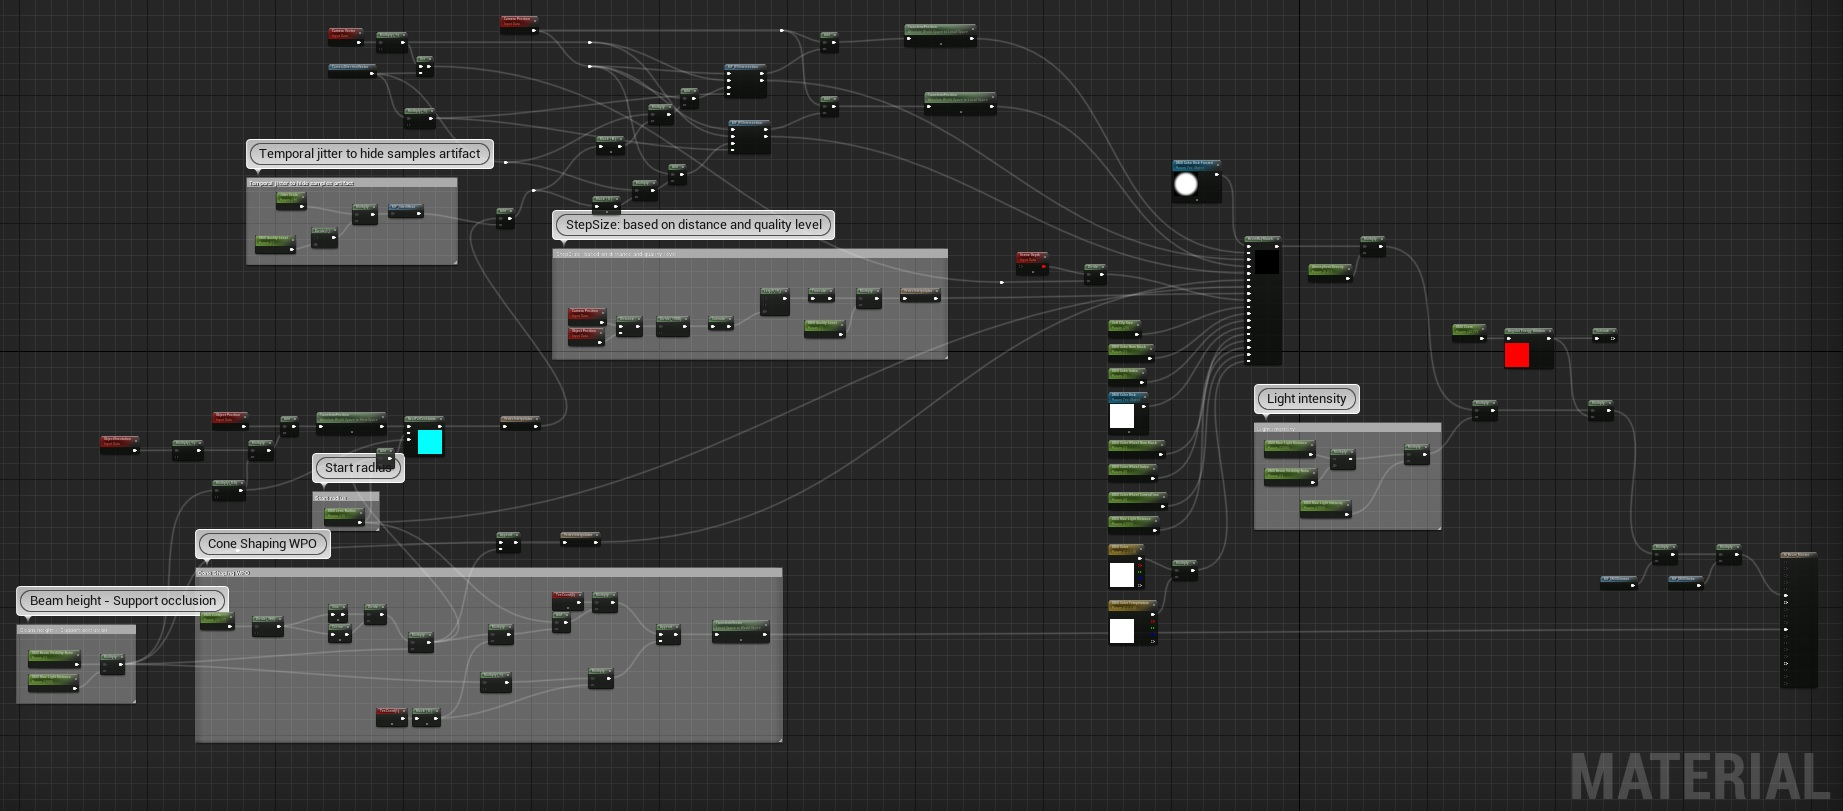
\includegraphics[width=1\linewidth]{img/renderingPipeline/BeamMaterialFull.jpg}
    \caption{Grafo del materiale Beam}
    \label{fig:2_beamGraphFull}
\end{figure}
Per renderizzare un beam, viene utilizzato l'algoritmo \say{Beam RayMarching}. In generale, gli algoritmi di RayMarching \cite{RayMarching} sono degli algoritmi per effettuare il sample di scene tridimensionali che vengono descritte in termini di \textit{SDF}, invece che esplicitamente con geometrie. SDF - \textit{Signed Distance Functions} - sono delle funzioni che ritornano la distanza minima tra un punto ed una superficie e che ci indicano, attraverso il segno, se tale punto si trovi all'interno o all'esterno della superficie stessa.\newline

\begin{wrapfigure}{r}{0.4\textwidth}
    \centering
    \captionsetup{justification=centering}
    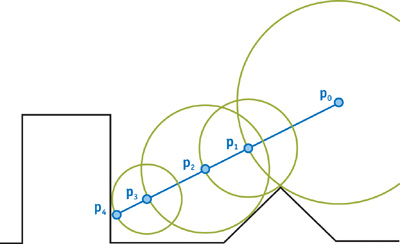
\includegraphics[scale=0.65]{img/renderingPipeline/spheretrace.jpg}
    \caption{Funzionamento dell'algoritmo di RayMarching}
    \label{fig:2_raymarchWikipedia} %taken from https://jamie-wong.com/2016/07/15/ray-marching-signed-distance-functions/
\end{wrapfigure}
Il Raymarching funziona lanciando, a partire dalla camera, un fotone per ogni pixel che deve renderizzare. Questo fotone, nell'implementazione standard, viene mosso iterativamente per un numero di step, fino a colpire un oggetto oppure fino alla fine delle iterazioni. La distanza percorsa ad ogni iterazione è uguale all'SDF tra la posizione del fotone all'iterazione precedente e la superfice della scena, in modo da essere sicuri di non registrare troppo tardi eventuali intersezioni.\newline

Il RayMarching viene spesso usato per generare geometrie che si ripetono, ed è esattamente come viene usato all'interno di questo materiale: per disegnare un beam viene effettuata una operazione di sample più volte, a distanze regolari, della forma della luce che vogliamo proiettare lungo i raggi che escono da una fixture. La distanza tra un sample e l'altro (così come il numero di sample), a differenza da una implementazione pura di Raymarching, varia in base alla distanza dalla telecamera e dalla qualità di rendering scelta. Più sample faremo e più la luce risulterà uniforme. 
\begin{figure}[H]
    \centering
    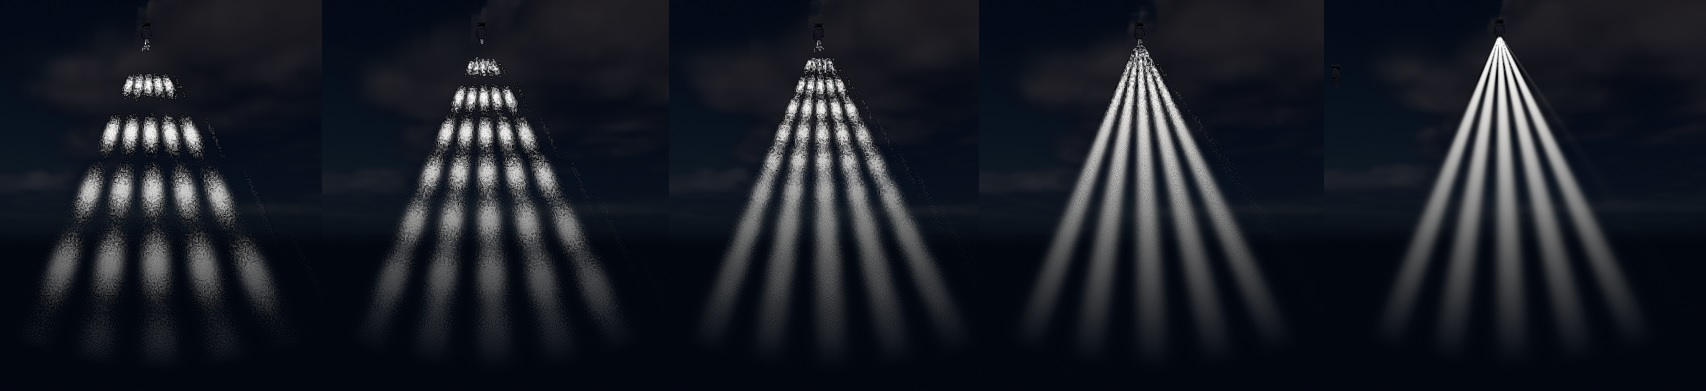
\includegraphics[width=1\linewidth]{img/renderingPipeline/renderingQuality.jpg}
    \caption{Diminuendo o aumentando il numero di sample si vede chiaramente come l'effetto beam sia ottenuto ripetendo la texture che vogliamo proiettare (4 punti in fila orizzontale) un numero elevato di volte.}
    \label{fig:2_raymarchQualities}
\end{figure}



\subsubsection{Light}\label{subsec:2_1_light}
Questo materiale si occupa della proiezione della luce su altri materiali
%TODO SCREENSHOT
Come possiamo notare è molto basilare, abbiamo due MaterialFunctionCall che si occupano dell'elaborazione del dimmer e della strobo, che vengono moltiplicati con il risultato di una terza MaterialFunctionCall chiamata \say{TODO}. Aprendo quest'ultima possiamo notare un grafo più interessante, che è quello con cui vengono renderizzate le ruote.
%TODO SCREENSHOT E SPIEGAZIONE
Da notare come il nome dei parametri all'interno di questa MaterialFunction facciano riferimento solo alle ruote gobo, e come all'interno del Materiale originale sia presente solamente una MaterialFunctionCall a questa MF. Questo implica l'impossibilità di renderizzare sia ruote differenti da quelle gobo e l'impossibilità di avere più ruote gobo nella stessa fixture

\subsubsection{Lens}\label{subsec:2_1_lens}
Questo materiale si occupa di applicare l'effetto che stiamo renderizzando sulle lenti (virtuali) di un faro %SCREENSHOT + EFFETTO SU LENTI VERE


\subsection{Idea della pipeline}\label{subsec:2_pipelineIdea}
Nelle precedenti sezioni abbiamo potuto vedere come allo stato attuale sia davvero difficile aggiungere nuove features e rendere possibile la presenza di più attributi contemporaneamente. Una buona idea per risolvere questi problemi è quella di astrarre il rendering dei vari moduli in moduli generici e realizzare una pipeline il più simile possibile ad una vera fixutre. Come spiegato in precedenza, in una vera luce è presente un emettitore che genera un fascio di luce che attraverserà ogni singolo modulo montato. Ogni singolo modulo prende quindi il \say{risultato} del modulo precedente, ci applica un filtro sottrattivo sopra e lo da in output al modulo successivo. \newline

La stessa identica cosa è stata quindi implementata su Unreal Engine. Verrà creata una nuova MaterialFunction contenente l'intera pipeline. Tutte le feature di una luce vengono trasformate in MaterialFunction che prenderanno in input, oltre ai loro parametri, il valore elaborato dalla precedente MF, e che daranno in output il valore modificato dalla feature. Tutte le feature che riguardano i colori (eccezion fatta della color wheel) verranno renderizzate al di fuori di questa catena di moduli (L'argomento verrà approfondito nel capitolo \ref{sec:FixtureComponentHierachy}) e l'output di questo processo verrà utilizzato come primo nodo della pipeline. L'output dell'ultimo nodo verrà collegato all'output della MaterialFunction. Ogni modulo della pipeline si occuperà, internamente, di fare il rendering della feature, invertirlo matematicamente, e poi sottrarlo al valore del nodo precedente. \newline
Questa MaterialFunction contenente la nuova pipeline verrà quindi piazzata al posto di quella che calcola le ruote gobo dentro il rendering Light e Lens, in modo da toccare il meno possibile i materiali originali. Nel contesto del materiale originale, è come se stessimo renderizzando una gobo molto elaborata e già colorata. \newline
E per il rendering del Beam?

\subsubsection{Problemi con le MaterialExpressionCustom e le MaterialFunction}\label{subsec:2_2_CM-MFproblems}
Come spiegato nella sezione \ref{subsec:2_1_beam}, il rendering del Beam di luce viene effettuato con una funzione di Raymarching scritta in HLSL dentro un blocco MaterialExpressionCustom. Purtroppo Unreal Engine non mette a disposizione un modo \say{pulito} per eseguire una MaterialFunction all'interno del codice di una MaterialExpressionCustom \cite{customExpressionMaterialFunction}. L'unica scelta rimane quindi di riscrivere l'implementazione dei vari moduli come funzioni in hlsl. Possiamo però dichiarare una funzione nel codice di una MaterialExpressionCustom? La risposta è no.
%TODO SCREENSHOT

Unreal Engine ci mette a disposizione tra i suoi vari menù, una finestra per consultare il codice HLSL che viene generato a partire da un Material. Andando a cercare ciò che abbiamo scritto nella MaterialExpressionCustom, notiamo che viene già inserita all'interno di una funzione.
%TODO CODICE

In C non si può dichiarare una funzione direttamente all'interno di un'altra funzione. Un modo per farlo però è quello di creare ed allocare una struct contenente all'interno le funzioni che vogliamo dichiarare. Utilizzando l'oggetto allocato è poi possibile andare effettivamente a chiamare le funzioni.
%TODO CODICE + SCREENSHOT DEL RISULTATO

Il motivo per cui si è preferito mantenere una doppia implementazione dei vari moduli (Sia come materiali che come codice HLSL) deriva dal fatto che quando Unreal Engine va a compilare i materiali in codice HLSL effettua una prima, grossa, ottimizzazione in cui eventuali valori e calcoli che non cambiano durante il rendering di un materiale vengono automaticamente messi in una cache. La stessa cosa non accade al codice HLSL dentro le MaterialExpressionCustom, che viene invece incapsulato senza essere toccato all'interno di una funzione, nel sorgente HLSL del materiale di cui fa parte. [TODO FIND REFERENCE]

\subsection{Generazione dinamica del codice e delle MaterialExpression}\label{subsec:2_codeGeneration}
\subsubsection{Custom Material (per Beam)}\label{subsec:2_3_CM}
\subsubsection{Material Function (per Light e Lens)}\label{subsec:2_3_MF}


\end{document}